\documentclass[UTF8]{ctexart}
\title{数据库开发技术实验报告}
\author{ljing12@software.nju.edu.cn ID.121250083 }
\date{Oct. 2014}

\usepackage{listings}
\usepackage{natbib}
\usepackage{graphicx}

\begin{document}
\maketitle
\section{Step 1}

建立一张包含四列的表,表名为test,第一列为id,主键,自增;第二列为col1,随机为Mike,
Bob,Jack,Alice,Cathy,Ann,Betty,Cindy,Mary,Jane中的一个;第三列为col2,随机为一个5位
字母序列,字母限制在\{a,b,c,d,e\};第四列为col3,随机为一个1-1000的整数。
    \begin{enumerate}
        \item 建表命令
        
        \textbf{create} \textbf{table} test(
        
        id \textbf{int}(10) \textbf{primary} \textbf{key} \textbf{auto\_increment},
        
        col1 \textbf{enum}('Mike','Bob','Jack','Alice','Cathy','Ann','Betty','Cindy','Mary','Jane'),

        col2 \textbf{char}(5),

        col3 \textbf{int}(4)
        );
        \item 约束的实现
        \begin{enumerate}
            \item 主键、自增和col1的随机姓名都由SQL提供的特性实现
            \item col2由高级语言实现,用java对插入的数据进行控制
        \end{enumerate}
        \item 实验平台说明
        \begin{enumerate}
            \item Operating System: Ubuntu 12.04
            \item DBMS: mysql-5.5.38-0ubuntu0.12.04.1
            \item default storage engine: InnoDB
        \end{enumerate}
    \end{enumerate}

\section{Step 2}
按照Step 1中对表的要求插入100万条记录,记录执行时间。
    \begin{enumerate}
        \item 最初步的想法是一条一条插入,代码如下
        \begin{figure}[ht]
            \centering
            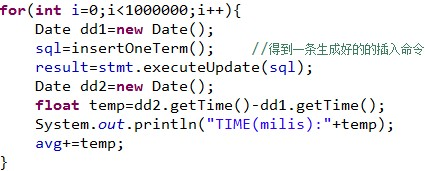
\includegraphics[scale=0.7]{db1.jpg}
            \label{fig:db1}
        \end{figure}

        实验结果:
        统计出平均每条插入时间约为194.9毫秒,也就是说100万条记录的插入需要消耗约
        54分钟时间,效率非常差
        \item 使用多条数据一个SQL语句的方法,减少SQL语句解析的时间。
        \begin{figure}[ht]
            \centering
            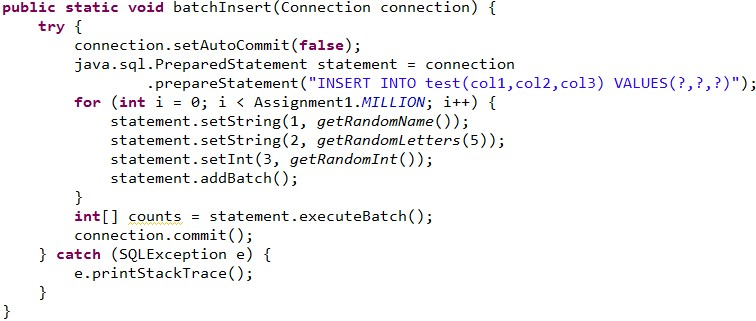
\includegraphics[scale=0.7]{db2.jpg}
            \label{fig:db2}
        \end{figure}

        实验结果:$Time=134893(ms)\approx135(s)$,效率明显提升。
        \item 使用\textbf{load data infile}操作,在java程序中,
            生成出data.txt文档,然后直接在mysql的命令行中导入
        \begin{figure}[ht]
            \centering
            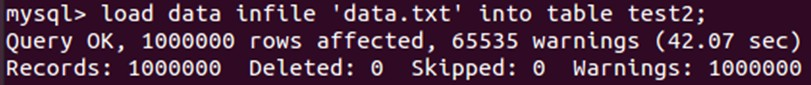
\includegraphics[scale=0.4]{db3.jpg}
            \label{fig:db3}
        \end{figure}

        可以看到即使加上生成数据文件和建立数据库连接的时间,这种做法依然是
        效率很高的一种做法,NICE!
    \end{enumerate}

\section{Step 3}
执行\textbf{select} count(*) from test \textbf{where} col3$>$=10
\textbf{group by} col1 \textbf{order by count}(*);记录执行时间。
    \begin{enumerate}
        \item 直接执行以上语句进行分析
        \begin{figure}[ht]
            \centering
            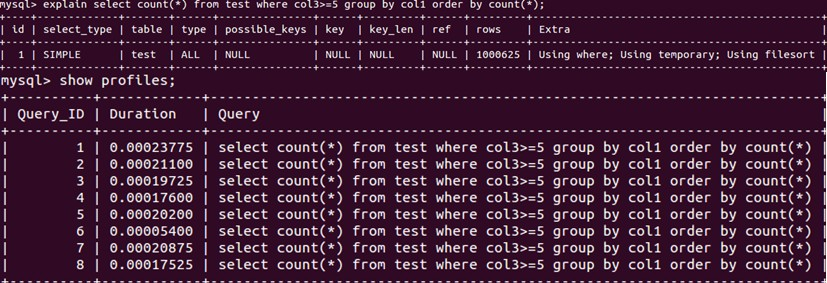
\includegraphics[scale=0.6]{db4.jpg}
            \label{fig:db4}
        \end{figure}

        分析Explain的结果,可以看出type是all,即没有使用索引而是全表遍历,Extra里面
        是where,这里面使得性能变慢的原因可能是Using temporary,因为临时没有索引,
        filesort可能导致性能变慢,如果要提高性能应该从这点入手。
        \item 使用所有进行优化,给col1,col3分别创建索引,如下
        
        \textbf{create index} index1 on test(col1);
        
        \textbf{create index} index3 on test(col3);
        \begin{figure}[ht]
            \centering
            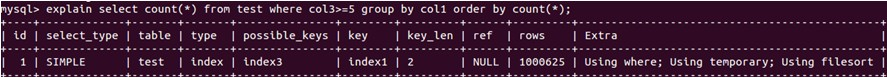
\includegraphics[scale=0.55]{db5.jpg}
            \label{fig:db5}
        \end{figure}
        
        可以看到,type一栏已经变成了index,即不再全表遍历,而是只扫描了索引,应该是有
        性能上的提高的,结果如下:
        \begin{figure}[ht]
            \centering
            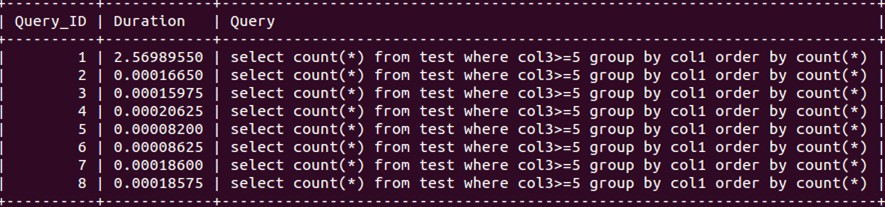
\includegraphics[scale=0.55]{db6.jpg}
            \label{fig:db6}
        \end{figure}
        
        但是从结果来看提升效果并不明显,我不怎么清楚原因。
        \item 另一种思路是降低count(*)扫描的行数,也就是把行数最多的部分使用索引来处理
            查询语句如下,把$>=$5转化为减去$<$5
            
            \textbf{select} cnt1-cnt2 \textbf{as} cnt from 
            
            (\textbf{select} \textbf{count(*) as} cnt1,col1 \textbf{from} test \textbf{group by} col1)T1,
            
            (\textbf{select count(*) as }cnt2,col1 \textbf{from} test \textbf{where }col3$<$5 \textbf{group by }col1) T2
            
            \textbf{where} T1.col1=T2.col1 \textbf{order by} cnt;
            
            结果如下图:
        \begin{figure}[ht]
            \centering
            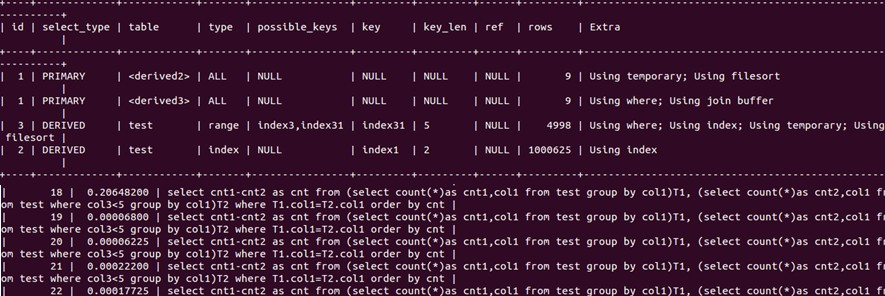
\includegraphics[scale=0.55]{db7.jpg}
            \label{fig:db7}
        \end{figure}    
        
        可以看到行数最多的部分是使用了index,而使用了temporary和filesort的行数很少,
        但是从结果上来说,数量级没有很明显的变化,也许是因为使用了子查询所以效率
        降低。
        \item 尝试改变了引擎为MyISAM,但是没有什么变化,查资料后发现,MyISAM对count(*)
            的性能神话有一个前提,是没有where语句,而这个查询中是有where语句的。
    \end{enumerate}

\section{Step 4}
找出所有col3不等于10的记录
    \begin{enumerate}
        \item 查询语句:
        \textbf{select }* \textbf{from }test \textbf{where }col3!=10;
        从Explain的结果来看,它没有使用索引,MySQL规定含有$<>$的是不
        使用索引的,运行时间约为$0.41s$左右,所以用
        \textbf{force index }强制它使用索引,结果如下:
        \begin{figure}[ht]
            \centering
            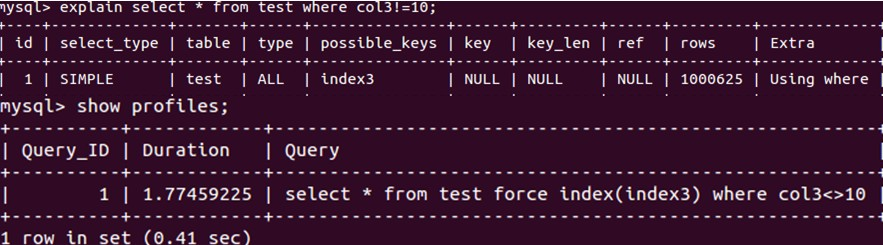
\includegraphics[scale=0.55]{db8.jpg}
            \label{fig:db8}
        \end{figure} 
        
        很明显,强制使用索引使得效果更差,这是因为此步骤中的SQL语句是一个不怎么
        适合使用索引的语句,因为它的结果集太大,反而是全表遍历比较节省时间。
        
        \item 相办法对一个更小的结果集进行操作,从而可以使用索引,SQL语句:
        
        \textbf{select * from }test \textbf{where }id \textbf{not in} 
        (\textbf{select } id \textbf{from }test \textbf{where} col3=10);
        \begin{figure}[ht]
            \centering
            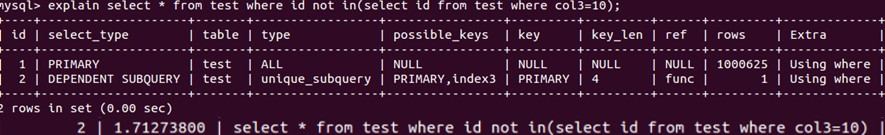
\includegraphics[scale=0.55]{db9.jpg}
            \label{fig:db9}
        \end{figure} 
        
        虽然子查询用了索引,结果仍旧不怎么好,还不如全表遍历。
        \item 用\textbf{select }* \textbf{from }test \textbf{where }col3$>$10;进行实验,是因为考虑到,$>$号产生的是范围查询,可能更适合
            使用索引一些,结果如下:
        \begin{figure}[ht]
            \centering
            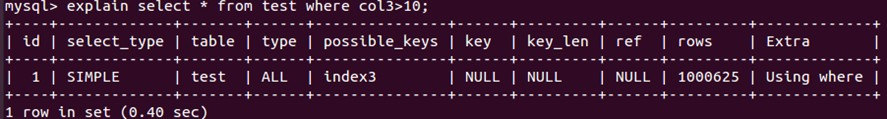
\includegraphics[scale=0.55]{db10.jpg}
            \label{fig:db10}
        \end{figure} 
        
        在这里,MySQL仍旧没有使用索引,强制使用索引之后,发现,和第一种思路强制
        使用索引结果一样,反而效率下降到了1.7s左右,这就说明这种结果集较大的情况
        最好还是尊重查询优化器的选择,让它全表遍历。
        
    \end{enumerate}

\section{Step 5}
找出所有第二列包含ab的记录,记录执行时间
    \begin{enumerate}
        \item \textbf{select }* \textbf{from }test \textbf{where }col2 \textbf{like } '$\% ab\% $';
        \begin{figure}[ht]
            \centering
            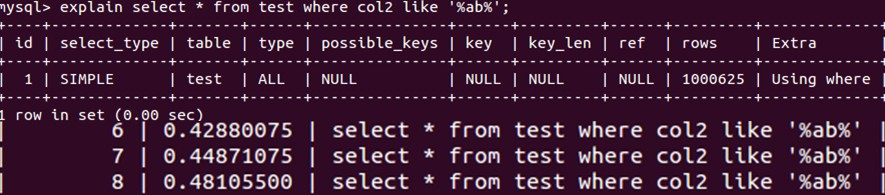
\includegraphics[scale=0.55]{db11.jpg}
            \label{fig:db11}
        \end{figure} 
        \item 尝试给col2加上索引
        \begin{figure}[ht]
            \centering
            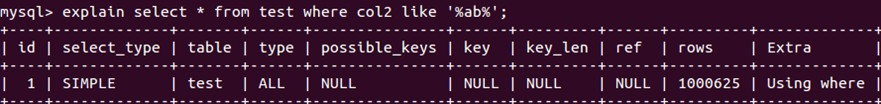
\includegraphics[scale=0.55]{db12.jpg}
            \label{fig:db12}
        \end{figure} 
        
        发现结果没有什么变化,执行时间也没有什么变化,和原来是一样的
        ,原因在于like '$\% ab\% $'是使用全表遍历,不使用索引,因为
        B树索引必须是从左到右最左端开始匹配的。
        
        \item 
        一种可能的解决方法是使用fulltext,在mysql 5.6+版本innodb已经支持fulltext索引,但是我的实验环境不支持,没有
        进行验证。
    \end{enumerate}
\section{Step 6}
找出所有第二列以ab开头的记录,记录执行时间
    \begin{enumerate}
        \item 
        \textbf{select }* \textbf{from }test \textbf{where }col2 \textbf{like } '$ab\% $';
        \begin{figure}[ht]
            \centering
            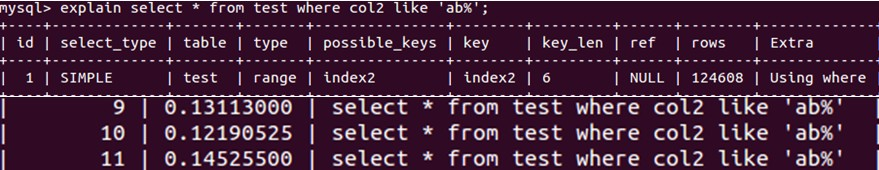
\includegraphics[scale=0.55]{db13.jpg}
            \label{fig:db13}
        \end{figure}
        
        可以看到,正如上面一道题目分析的一样,当最左端匹配的时候,就使用了索引。
        \item 尝试给test表的col2列加上前缀索引,降低索引字段的长度
        
        \textbf{create index} index2 \textbf{on} test(col2(2));
        \begin{figure}[ht]
            \centering
            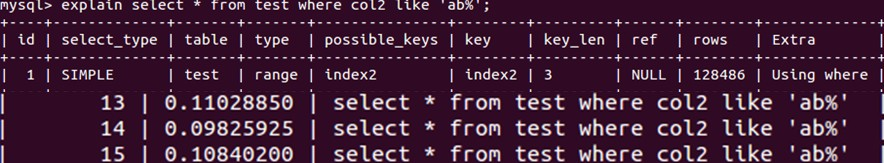
\includegraphics[scale=0.55]{db14.jpg}
            \label{fig:db14}
        \end{figure}
        
        可以看到结果还是有一定提高的
        
        
    \end{enumerate}

\section{Step 7}
模拟对数据库的并发操作,使用5个进程同时对数据库进行操作,查看效果
%\citep{ref7}

\bibliographystyle{plain}
\bibliography{database_tech_as1}
\end{document}
